\documentclass{article}
\usepackage{graphicx} % Required for inserting images
\usepackage{listings}
\usepackage[margin=0.9in]{geometry}
\usepackage{indentfirst}
\usepackage{float}
\usepackage{hyperref}

\title{\Huge CTA200 final project}

\author{Areeba Khan}
\date{May 2026}

\begin{document}

\maketitle

\newpage
\section{ Retrieving EAGLE Galaxy properties} % section 1
    %------------------------------------------------------
\subsection{Setup} %1.1
Python based tools for using the EAGLE SQL database were installed using the \texttt{pip install eaglesqltools} command.
    %------------------------------------------------------
\subsection{} %1.2
The first query was made:
\begin{verbatim}
query="""SELECT MassType_Star as stellar_mass,
StarFormationRate as SFR
FROM RefL0100N1504_SubHalo
WHERE SnapNum = 28"""
\end{verbatim}
This outputs the column ``MassType\_Star'' by renaming it as ``stellar\_mass'', and ``StarFormationRate'' by renaming it as ``SFR''. The ``FROM'' clause is just to tell SQL which database to get these columns from, which in this case is ``RefL0100N1504\_SubHalo''. The ``WHERE'' clause puts a condition and specifies which rows to get the information from. It acts like a filter--choosing only those rows where the ``SnapNum'' is equal to the number 28. 

Overall, the rows with SnapNum=28 will be chosen from the database ``RefL0100N1504\_SubHalo'', and only two columns--``stellar\_mass'' and ``SFR''--will be output. The resulting table will have two columns, and all the rows where SnapNum=28.
The same constraint of SnapNum =28 could also be made by editing the ``WHERE`` clause by writing \texttt{WHERE redshift = 0}
    % -------------------------------------------------------
\subsection{} %1.3
Next, plots of the data retrieved were made using \texttt{matplotlib} to inspect it. The columns of the data that was retrieved were indexed using the names given in the first query. A simple scatter plot was made by switching the axes to logarithmic scales for a more even figure. It was found that in this snapshot, there were 2,275,510 galaxies.
\begin{figure}[H]
    \centering
    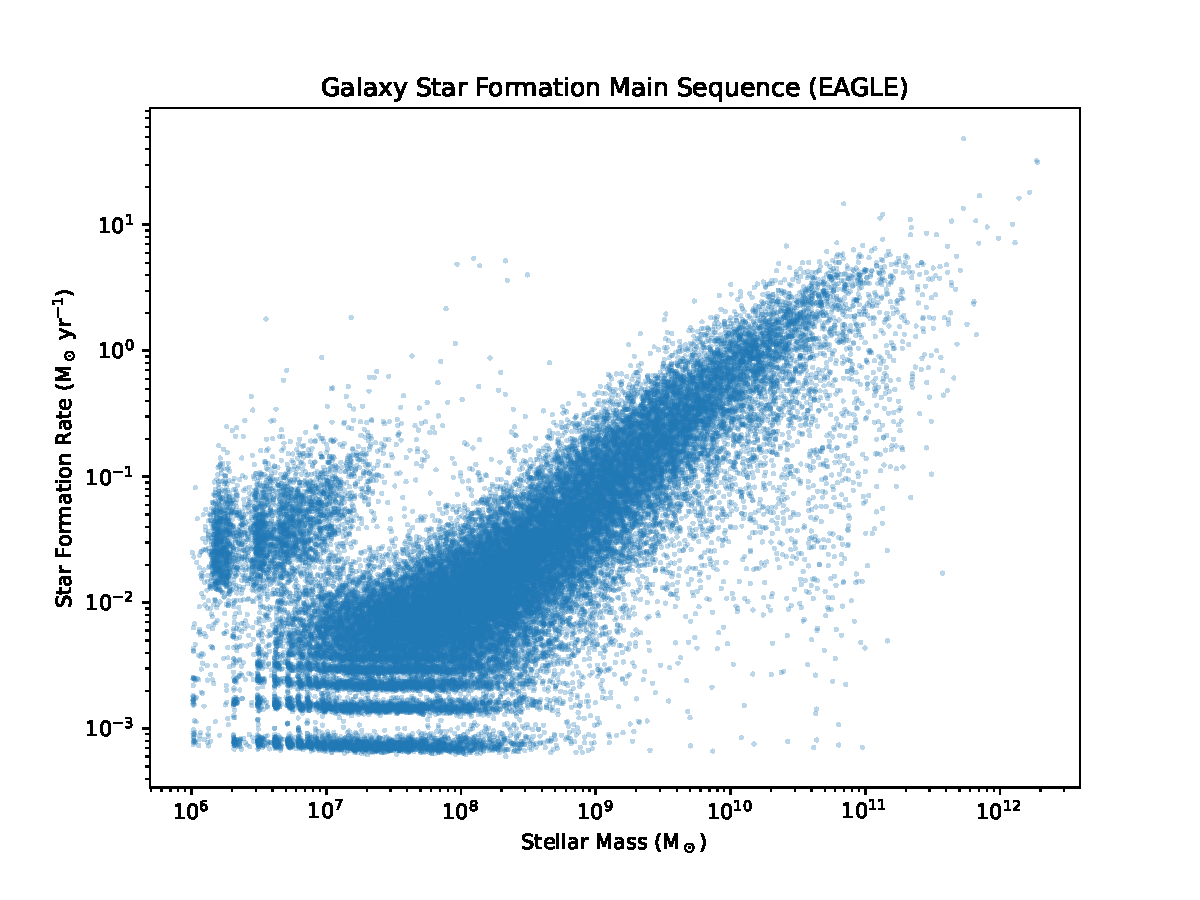
\includegraphics[width=0.7\textwidth]{eagle_scatter.pdf}
    \caption{Scatter plot of Stellar Mass and Star Formation Rate from EAGLE data}
    \label{fig:my_picture}
\end{figure}
Similarly, a histogram was made by filtering out zeros for log scale, and a plot showing the line of best fit along with its standard deviation was made to inspect the data.
% histogram
\begin{figure}[H]
    \centering
    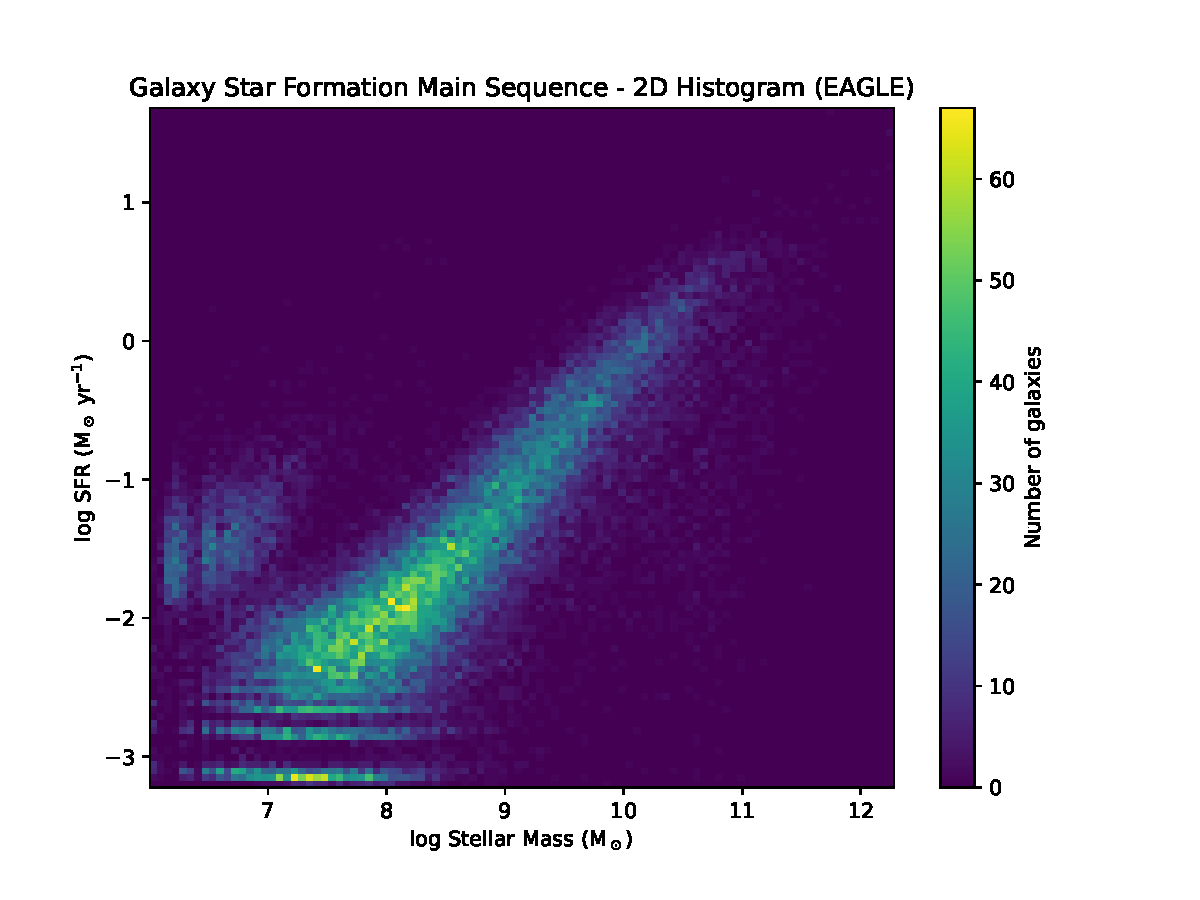
\includegraphics[width=0.8\textwidth]{eagle_histogram.pdf}
    \caption{Histogram of Stellar Mass and Star Formation Rate from EAGLE data}
    \label{fig:my_picture}
\end{figure}

%line of best fit stuff
\begin{figure}[H]
    \centering
    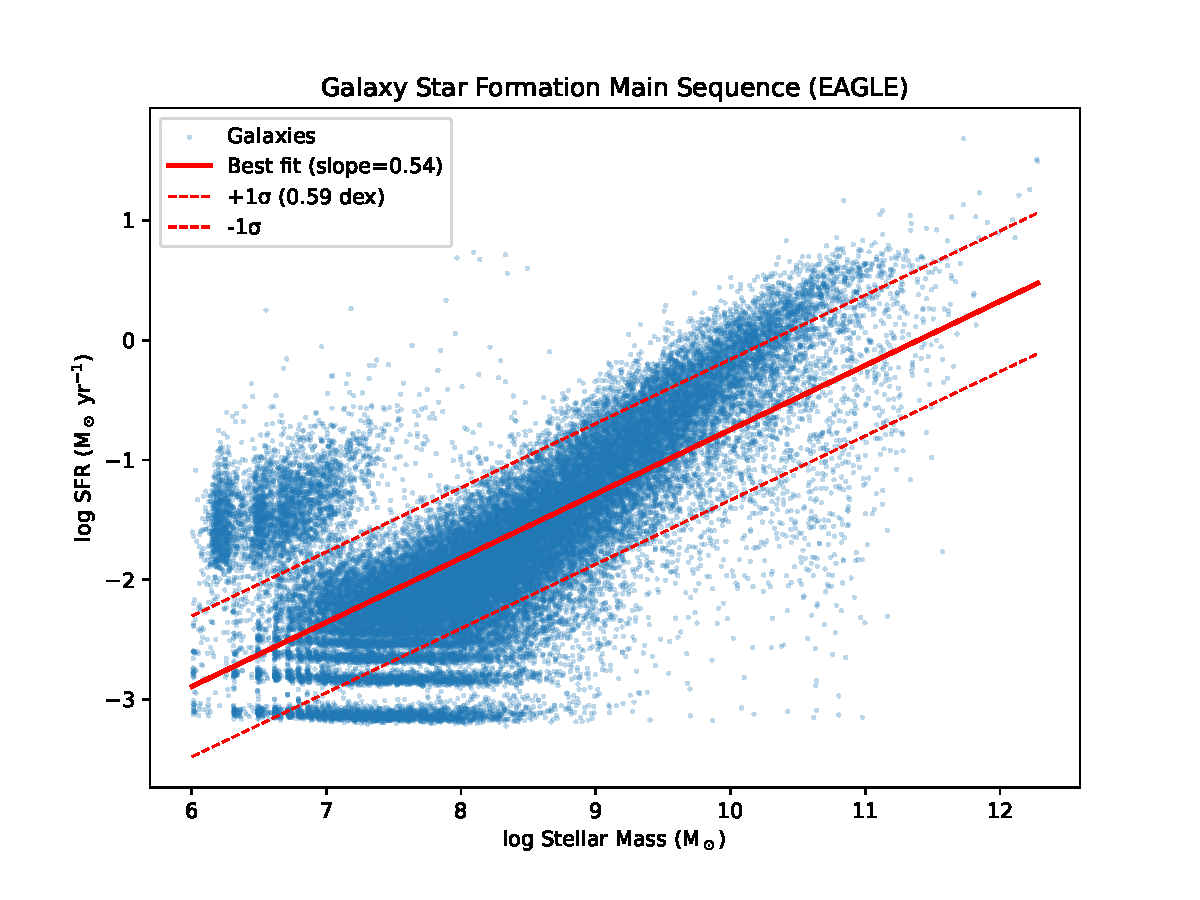
\includegraphics[width=0.8\textwidth]{eagle_scatter_bestfit.pdf}
    \caption{Plot showing line of best fit along with the standard deviation}
    \label{fig:my_picture}
\end{figure}
    %--------------------------------
\subsection{} % 1.4
From Figure 1, it can be seen that the relationship is roughly linear. Meaning, galaxies with higher stellar mass typically have higher star formation rates (Alton, 2016). This is known as the "galaxy star formation main sequence" (Mackereth and Savelli, 2026). This shows that for most other galaxies in the universe, the star formation process is steady and self-regulating. Galaxies that have more stars tend to have more gas available to keep forming new stars. Additionally, a galaxy’s current star formation rate is dependent on its history of star formation (Alton, 2016).

Although the plot gives a good idea of the relationship between stellar mass and SFR, there are a number of features of this distribution that are very different to what one sees in nature. The low stellar mass end of the plot has almost no galaxies-- it is empty, and the data points start at about $10^6 M_{\odot}$ all of a sudden. This is due to the fact that the minimum stellar mass in the simulation is higher compared to reality where there are at least a few low-mass galaxies. The reason for that is because simulations like EAGLE have minimum particle mass resolution, meaning small low mass galaxies can not be modelled. This enables EAGLE to run large volume simulations because it doesn’t need to resolve any tiny galaxy.

Additionally, in the figure a cloud of data points showing galaxies with very high stellar mass but low star formation rate can be seen. These are quenched galaxies which have stopped forming stars (Alton, 2016). In the real universe, these are red galaxies. Also, the straight horizontal lines seen in the plot are quite unusual; these discrete lines are not physical because SFR should be continuous. The reason for this is mainly the resolution limit of EAGLE simulation where SFR is calculated from discrete gas particles with only certain allowed minimum values. Similarly, there is a cluster of data points around stellar mass $10^6 - 10^7 \, M_{\odot}$, which is again due to the resolution limit of the simulation. Since there is a minimum threshold, many galaxies seem to suddenly pile up near those points.
%-------------------------------------------------------------------
% section 2 
\section{Going Deeper into the Simulations: more properties and more
snapshots} 
\subsection{}  % 2.1 section
The simulation data in the EAGLE database covers a number of different snapshots of the simulations. The overall properties of galaxies derived from various particles are also computed at every snapshot. In the previous section, only the final output was looked at (where SnapNum=28), but this can be changed to look at a wider range of outputs. In this section, all galaxies found in snapshots after a redshift of 0.5 were analyzed. This is the range of redshifts from 0 $< z < 0.5$.

\begin{figure}[H]
    \centering
    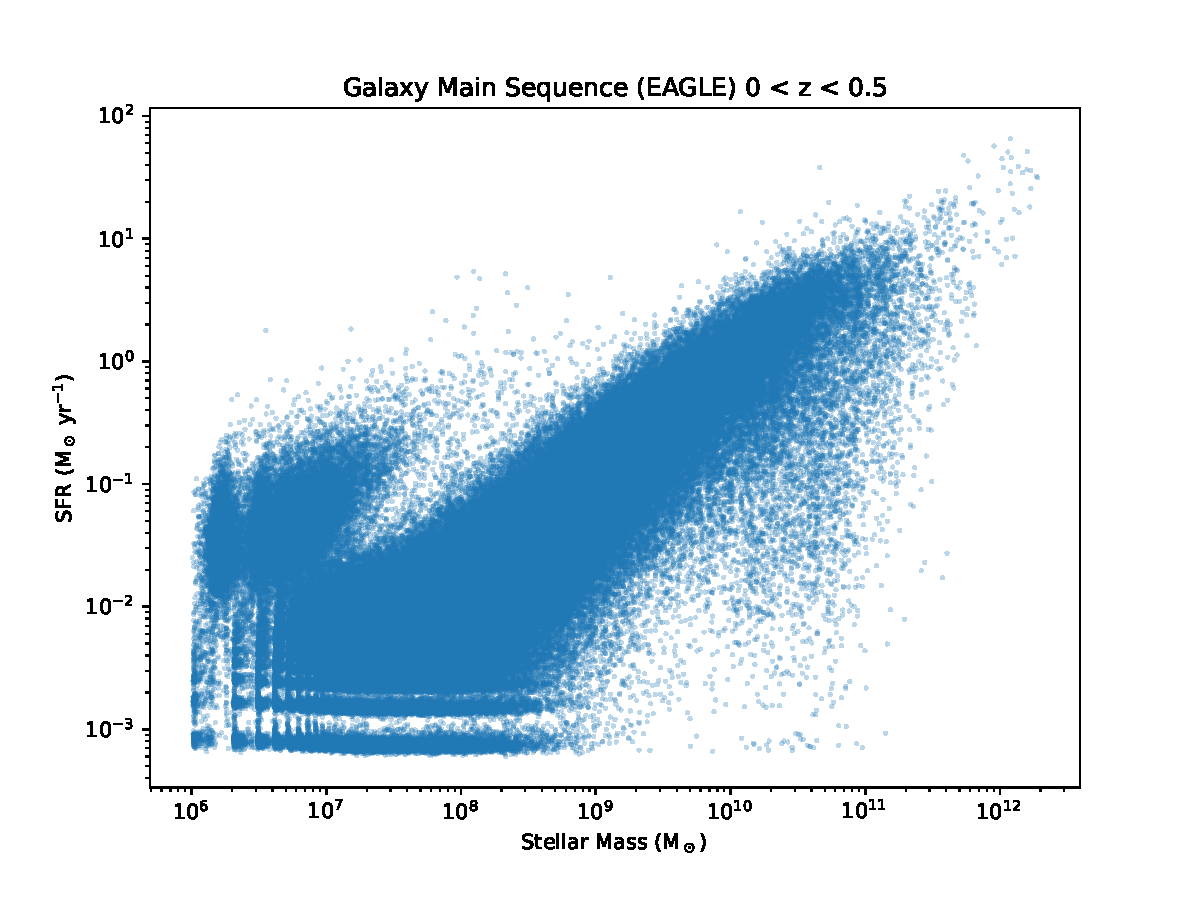
\includegraphics[width=0.8\textwidth]{eagle_scatter_z05.pdf}
    \caption{Stellar Mass vs SFR plot for redshifts 0 to 0.5}
    \label{fig:my_picture}
\end{figure}

It was found that there were 11,819,412 galaxies in this range of snapshots, which is significantly higher than the number of galaxies found in the previous section which was 2,275,510. Comparing both plots, it can be seen that Figure 4 has significantly more data points than Figure 1. It can also be seen that Figure 4 has more galaxies in the high stellar mass with higher SFR region compared to Figure 1. This is due to the fact that at earlier times (higher redshifts), massive galaxies were still actively forming stars that had not been quenched yet.
    %-------------------------------------------------------
\subsection{} %2.2
Selecting galaxies in this way is more representative of what one would see in an observational galaxy survey looking out from milky way. When observing the universe through a telescope, galaxies are not looked at a specific moment in time, rather at varying distances. This is due to the fact that light takes time to travel and reach the observer’s eye. Distant galaxies appear as they did in the past. Due to this, selecting galaxies from $0 < z < 0.5$ mimics what a real telescope would see in real life. The brightness of a galaxy determines the maximum redshift a survey can see, meaning, the farther a galaxy is, the fainter it would appear. Thus, the maximum redshift depends on the sensitivity / power of the telescope and the brightness of the galaxy. 

    %----------------------------------------------------------
\subsection{} % 2.3 -- optional but i'm doing it
Selecting multiple snapshots extracts information from the same galaxy across different times. In this section, the most massive galaxy and its direct descendants were isolated at z=0. To achieve this, the EAGLE database was queried, ordering galaxies by stellar mass and selecting the top result at SnapNum=28. It was found that the most massive galaxy had a stellar mass of $\sim 1.9 \times 10^{12} \, M_{\odot}$ with GalaxyID = 21379521. using the merger tree structure described in Mcalpine et al. (2016), the main branch descendants were isolated by querying all galaxies with a GalaxyID between the galaxy's GalaxyID and TopLeafID. This traced the galaxy's direct lineage backwards in time from $z=0$ to $z=10$.
\begin{figure}[H]
    \centering
    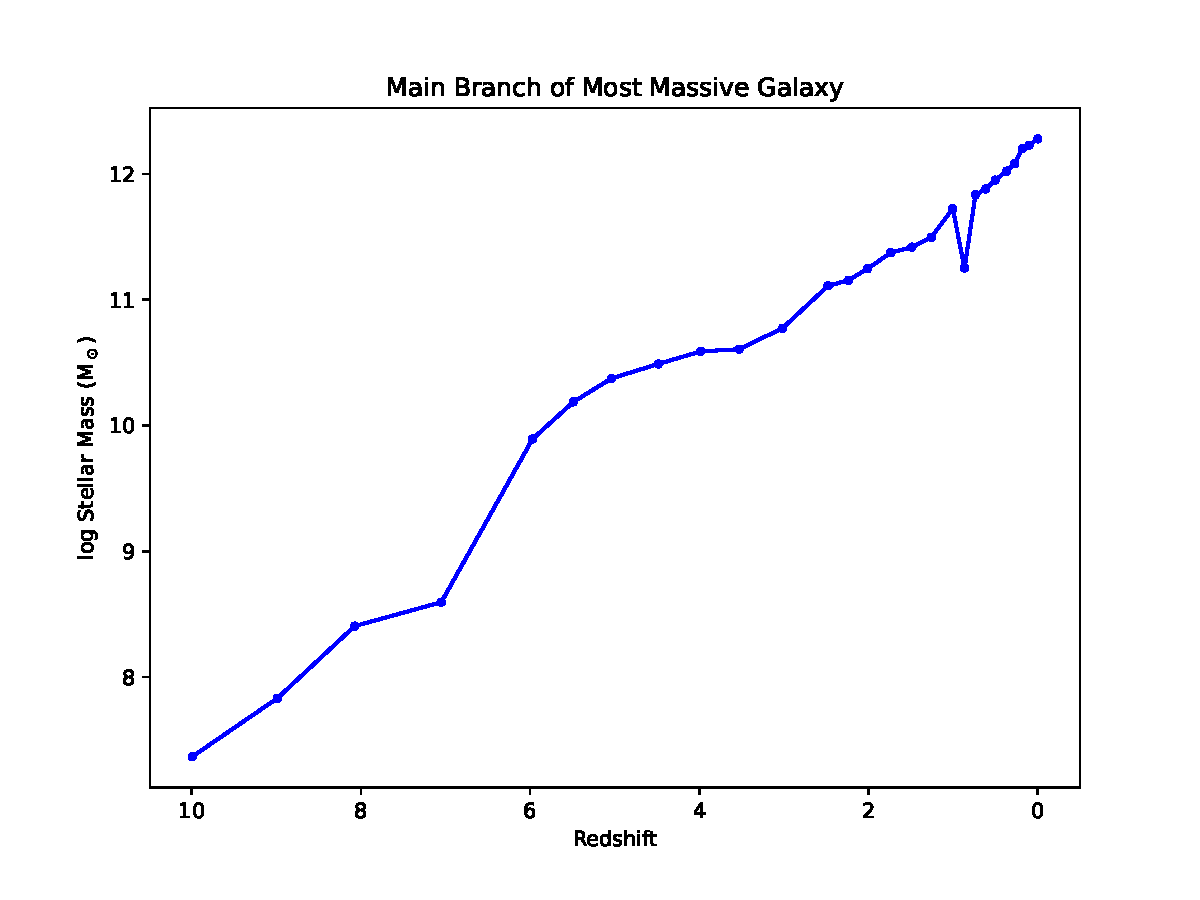
\includegraphics[width=0.8\textwidth]{mainbranch.pdf}
    \caption{Main branch of the most massive galaxy found}
    \label{fig:my_picture}
\end{figure}
Figure 5 shows the stellar mass growth history of this galaxy along its main branch. the galaxy grows steadily from $\sim 10^7 \, M_{\odot}$ at $z \sim 10$ to $\sim 10^{12} \, M_{\odot}$ at $z = 0$, reflecting continuous mass assembly through star formation and mergers. A notable dip is visible around $z \sim 2$ to $3$, which may indicate a major merger event where the main branch temporarily switches to a different descendant.

The number of galaxies in the main branch were 28. These galaxies along the main branch had the galaxy IDs;
\begin{verbatim}
[21379521 21379522 21379523 21379524 21379525 21379526 213579527 21379528
 21379529 21379530 21379531 21379532 21379533 21379534 21379535 21379536
 21379537 21379538 21379539 21379540 21379541 21379542 21379543 21379544
 21379545 21379546 21379547 21379548]
\end{verbatim}
    %---------------------------------------------------
% not doing 2.4 since its optional
%-----------------------------------------------------
\section{Another Simulation: Querying data from IllustrisTNG}
\subsection{} %3.1
In this section, the database was queried using a different set of simulations-- the IllustrisTNG project. Since TNG does not use SQL like EAGLE, API (Application Programming Interface) was used to access the data. A helper function was used whose purpose was to make a HTTP GET request to a specified URL. The response was saved in a python dictionary. 
    %----------------------------------------------------------
\subsection{}  % 3.2
All of the galaxies at redshift $z=0$ in the TNG100-1 were looked at. The response to the code was a dictionary object. The keys were explored to find out how many galaxies there were at $z=0$ in the simulation. TNG100-1 returned 4,371,211 while EAGLE had returned 2,275,510 subhalos at z=0. The difference in counts reflects differences in simulation volume, resolution, and how each simulation defines and counts subhalos, rather than a physical difference in the number of galaxies in the universe.

    %-----------------------------------------------------------
\subsection{} % 3.3
The initial data pull grabs only the first 100 galaxies. To get all galaxies, the code recommended was \verb|subhalos = get(z0url, {'limit':n_gal})| as per instructions, however, that command requested it to return 4+ million subhalos in one request which is way too many. The solution was not to loop over every single subhalo individually, and instead use TNG's bulk download feature by requesting only the fields that were needed with a limit on stellar mass. The modified code that was run was:
\begin{verbatim}
    # Limit to galaxies with some stellar mass to keep it manageable
    subhalos = get(z0url, {'limit': 50000, 'mass_stars__gt': 0.01})
    n_gal = len(subhalos['results'])
    print(f"Number of galaxies retrieved: {n_gal}")
\end{verbatim}
The \texttt{mass\_stars\_\_gt} filter means "stellar mass greater than 0.01" which cuts out the tiny dark matter halos with no stars — similar to what EAGLE was implicitly showing. This also made the main sequence plot much cleaner and directly comparable to the EAGLE plot. The limit was set to 50,000 as seen in the code, and the number of galaxies retrieved was 47928. Since this number is lesser than 50000, it was confirmed that all the galaxies were retrieved.
    %-----------------------------------------------------------
\subsection{}  % 3.4
A plot similar to what was made in Section 1 and Section 2 was made. However since there were 47,928 galaxies, the URL request would have run for hours. To fix this issue, the number of galaxies to be plotted was reduced to only 1000, which took about 15 minutes to run. The purpose of this was to get enough data points to see the overall trend, while also keeping time constraint in mind.

\begin{figure}[H]
    \centering
    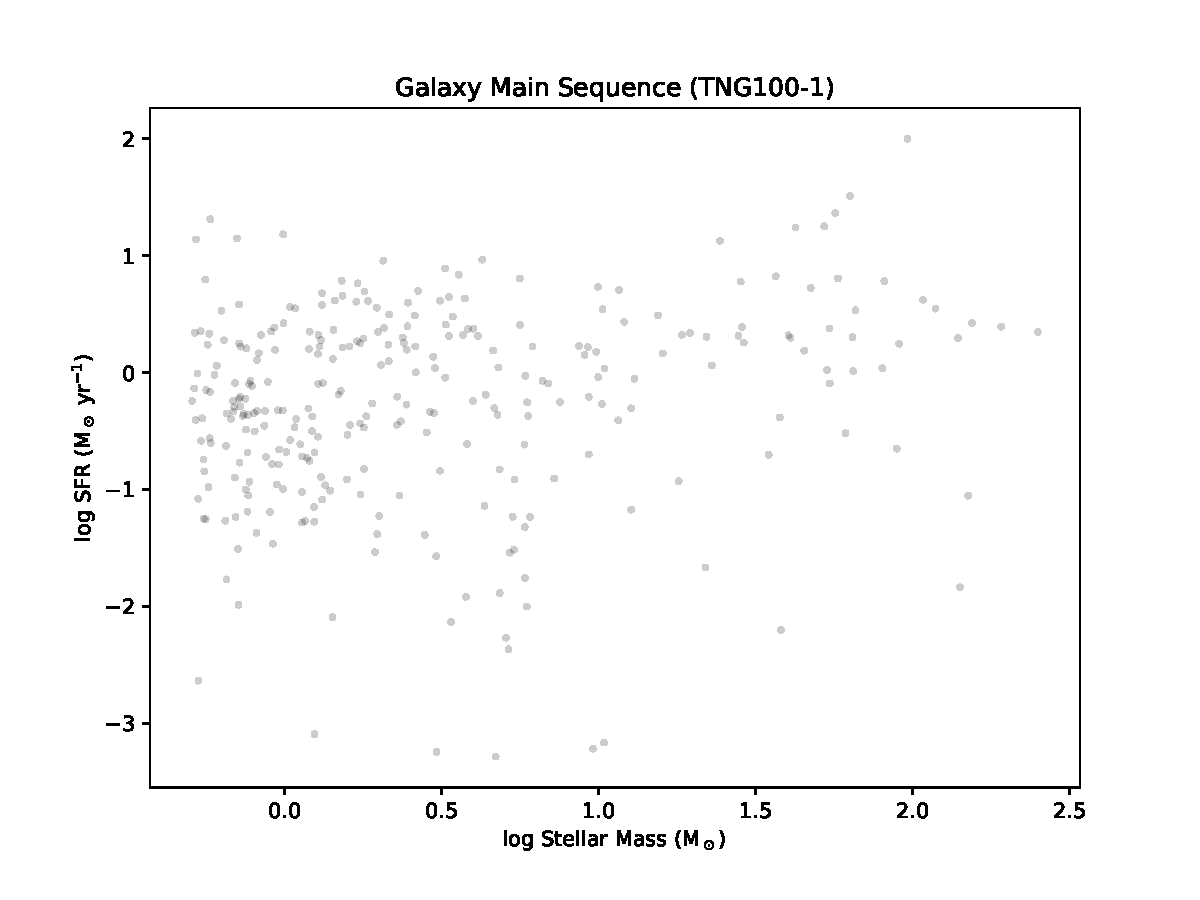
\includegraphics[width=0.8\textwidth]{TNG_scatter.pdf}
    \caption{Stellar mass vs SFR using TNG data}
    \label{fig:my_picture}
\end{figure}

Observing both Figure 6 and Figure 1, apart from the obvious (fewer data points) difference, there are a few differences between the plots. Figure 1, having data retrieved from EAGLE, has x-axis that goes from $10^6 - 10^{12}$ whereas the TNG x-axis goes from -0.5 to 2.5 in log. This is because TNG returns mass in units of $10^{10} \, M_{\odot}$ and not raw solar masses. Secondly, in EAGLE, SFR rising with stellar mass is very noticeable, whereas in the TNG plot the points are very scattered. This could be due to the small sample size, but it is worth noting that even with 1000 points, a basic trend is not easy to spot. 
Lastly, In EAGLE, quenched ("red and dead") galaxies have exactly zero SFR, so they get removed by the mask and are completely invisible in the plot. This is partly a numerical artifact of how EAGLE implements star formation — below a certain threshold it just sets SFR to zero.
In TNG, those same quenched galaxies still show up in the plot with very low but nonzero SFR (the points scattered at the bottom, around log SFR = -3). This means TNG retains more of the "red and dead" population visibly in the plot.
So the practical implication is: EAGLE likely underrepresents quenched galaxies in this plot, while TNG shows them more explicitly. In reality, red and dead galaxies make up a significant fraction of massive galaxies in the universe, so TNG's representation is arguably more physically realistic in this regard — though both simulations are approximations of the true quenching physics driven by AGN feedback.

\clearpage % Forces the bibliography to start on a new page

\begin{thebibliography}{9}

\bibitem{mcalpine2016}
McAlpine, S., Helly, J. C., Schaller, M., Trayford, J. W., Qu, Y., Furlong, M., Bower, R. G., Crain, R. A., Schaye, J., Theuns, T., Dalla Vecchia, C., Frenk, C. S., McCarthy, I. G., Jenkins, A., Rosas-Guevara, Y., White, S. D. M., Baes, M., Camps, P., \& Lemson, G. (2016). 
The EAGLE simulations of galaxy formation: Public release of halo and galaxy catalogues. 
\textit{Astronomy and Computing}, \textit{15}, 72--89. 
\url{https://doi.org/10.1016/j.ascom.2016.02.004}
%new line
\bibitem{mackereth2026}
Mackereth, T., \& Savelli, A. (2026, May 7). 
\textit{CTA200H Mini-Project: MW Analogues in cosmological simulations by Activity}. 
[Course Project].
% new line
\bibitem{alton2016}
Alton, P. (2016, November 10). 
The end of the line. 
\textit{Astrobites}. 
\url{https://astrobites.org/2016/11/10/the-end-of-the-line/}


\end{thebibliography}








\end{document}
